%%%%%%%%%%%%%%%%%%%%%%%%%%%%%%%%%%%%%%%%%%%%%%%%%%%
%
%  New template code for TAMU Theses and Dissertations starting Fall 2016.  
%
%
%  Author: Sean Zachary Roberson
%  Version 3.17.09
%  Last Updated: 9/21/2017
%
%%%%%%%%%%%%%%%%%%%%%%%%%%%%%%%%%%%%%%%%%%%%%%%%%%%

%%%%%%%%%%%%%%%%%%%%%%%%%%%%%%%%%%%%%%%%%%%%%%%%%%%%%%%%%%%%%%%%%%%%%%
%%                           SECTION I
%%%%%%%%%%%%%%%%%%%%%%%%%%%%%%%%%%%%%%%%%%%%%%%%%%%%%%%%%%%%%%%%%%%%%


\pagestyle{plain} % No headers, just page numbers
\pagenumbering{arabic} % Arabic numerals
\setcounter{page}{1}


\chapter{\uppercase {Introduction}}
%% What is the problem? 

%% Why is it hard? 
%% What have others done? 
%% What have I done?

\section{Topological quantum computation}

Topological quantum computation refers to a variety of proposals for building a quantum computer using topological phases of matter.  In the usual setup, one creates $n$ quasiparticle excitations (anyons) in a 2-dimensional disk.  Physically braiding quasiparticle excitations corresponds to a unitary action of the braid group $B_n$ on the Hilbert space of possible states of the system.  These unitary braid group representations are completely determined by the anyon types of the $n$ quasiparticles. The images of the standard braid group generators in such a representation form the gate set for a quantum computer.  

%% FIXME: Insert braiding PICTURE

More generally, we consider a system of quasiparticle excitations on a closed surface of arbitrary genus.  In this case, there may be nontrivial self-homeomorphisms of the underlying surface in addition to motions of the quasiparticle excitions on the surface.  Both types of actions correspond to elements of the mapping class group of a compact surface with boundary, where a labeled boundary component replaces each quasiparticle excitation. The aforementioned braid group example corresponds to the mapping class group of a disk with $n$ open disks removed, holding the outer, vacuum-labeled boundary fixed.  

\subsection{Topological quantum field theories}
The relevant dynamics of proposed topological phases of matter are governed by topological quantum field theories (TQFTs). The theories we consider in this paper are $(2+1)$-dimensional (two spatial dimensions and one time dimension). A $(2+1)$-dimensional topological quantum field theory assigns a vector space to every oriented compact surface and a (possibly projective) linear map to every $3$-manifold with boundary in a compatible way.  In particular, if a $3$-manifold $M$ has boundary $\partial M = N_1 \sqcup \overline{N_2}$, then a TQFT $F$  defines a (projective) operator $F(M) : F(N_1) \to F(N_2)$.   Specializing to the case where $N := N_1 = N_2$, a TQFT defines a representation of the mapping class group of $N$.

%% FIXME: cite RT construction
A common way of constructing TQFTs is by labelling geometric data (e.g. simplices of a triangulation, or framed links) by data from a sufficiently nice tensor category.  Two such constructions are the Reshitikhin-Turaev \cite{reshetikhin1991invariants} and the Turaev-Viro-Barrett-Westbury \cite{hep-th/9311155, TURAEV1992865} constructions.

More concretely, given a spherical fusion category $\mathcal A$ over a field $k$ and an oriented compact surface $\Si$, possibly with boundary, the Turaev-Viro-Barrett-Westbury (TVBW) construction gives a projective representation of the mapping class group $\MCG(\Si)$ \cite{hep-th/9311155, TURAEV1992865}. A natural problem motivated by topological quantum computation is to determine the images of such representations.  In particular, we would like to know when such a representation has a finite image.

%% \subsection{Spherical fusion categories}

%% The algebraic aspects of two dimensional topological phases of matters are governed by the theory of fusion categories. A fusion category is a rigid semisimple linear monoidal category with only finitely many isomorphism classes of simple objects.  Each anyon type corresponds to an isomorphism class of simple objects.

%% %% TODO:
%% % \subsubsection{Monoidal categories}
%% %% A monoidal category is a triple $(\mC, \otimes, 


\section{The Property F conjecture}
It is conjectured that any TVBW mapping class group representation associated to a spherical fusion category $\mathcal A$ has finite image if and only if  $\mathcal A$ is weakly integral.  This conjecture is a modification of the Property F conjecture \cite{erw, nr}, which states that braid group representations coming from a braided monoidal category $\mathcal C$ should have finite image if and only if $\mathcal C$ is weakly integral. Instead of only considering braid group representations, one can consider mapping class groups of arbitrary orientable surfaces.  In this case, the input categories to construct the representations must be more specialized than just braided monoidal.  One can either apply the Reshitikhin-Turaev construction to a modular tensor category, or apply the TVBW construction to a spherical fusion category.  The former is more general than the latter since the Reshitikhin-Turaev construction for the Drinfeld center $Z(\mathcal A)$ of a spherical fusion category $\mathcal A$ yields the same representation as the TVBW construction for $\mathcal A$.  However, for the case considered in this paper, the simpler TVBW construction suffices.

In this paper, our input category is  $\mathcal A = \Vect_G^\omega$, the spherical fusion category of $G$-graded vector spaces with associativity modified by a cocycle $\omega \in Z^3(G, k^\times)$.  In this case, the TVBW construction corresponds to both twisted Dijkgraaf-Witten theory \cite{dijkgraaf1990} and the Reshitikhin-Turaev construction \cite{reshetikhin1991invariants} applied to $\Mod-D^\omega(G) \cong Z(\Vect_G^\omega)$.  The category $\Vect_G^\omega$ is integral, so the one expects its associated mapping class group representations to have finite image.  The main contribution of this paper is to verify this for arbitrary $G$ and $\omega$.



%% TODO: \subsection{Universality}
%% TODO: \subsection{Weak integrality}
%% TODO: \subsection{Current progress}

\subsection{The spherical fusion category $\Vect_G^\omega$}
The following definitions are well-known and can be found in, e.g., \cite{etingofTensor}.  Let $k$ be an algebraically closed field of characteristic 0,  $G$ a finite group, and $\omega \in Z^3(G, k^\times)$ a 3-cocycle.    The spherical fusion category of $G$-graded $k$-vector spaces with associativity defined by $\omega$ is denoted $\Vect_G^\omega$.  The objects of this category are vector spaces with a decomposition $V = \bigoplus_{g \in G} V_g$. Morphisms are linear maps preserving the grading. The tensor product is defined by
$$ (V \otimes W)_g = \bigoplus_{x,y \in G, xy = g} V_x \otimes W_y. $$

For each $g \in G$, pick a 1-dimensional vector space $\delta_g \in \Obj(\Vect_G^\omega)$ concentrated in degree $g$.  The set $\{\delta_g : g \in G\}$ is a complete set of pairwise non-isomorphic representatives for the isomorphism classes of simple objects of $\Vect_G^\omega$.  We will sometimes abuse notation by referring to an object $\delta_g$ by the group element $g$.  We have $\one \cong \delta_1$, and  $\delta_g^* := \delta_{g^{-1}}$ with the coevaluation and evaluation maps defined below.

For the structural morphisms,  we follow \cite{math/0601012}.  We will treat the canonical isomorphisms $\delta_g \otimes \delta_h \cong \delta_{gh}$ as identities.    The associator $\alpha_{g,h,k}:(\delta_g \otimes \delta_h) \otimes \delta_k \to \delta_g \otimes (\delta_h \otimes \delta_k)$ is defined by
$$\alpha_{g,h,k} = \omega(g,h,k) \id_{ghk}.$$ 
The evaluation $\ev_g:\delta_g^* \otimes \delta_g \to 1$ is 
$$\ev_{g} = \omega(g^{-1},g,g^{-1}) \id_1.$$  
The coevaluation $\coev_g:1 \to \delta_g \otimes \delta_g^*$ is 
$$\coev_{g} = \id_1.$$ 
The pivotal structure $j_g:\delta_g \to \delta_g^{**}$ is 
$$j_{g} = \omega(g^{-1},g,g^{-1}) \id_{g}.$$

If $\omega$ and $\omega'$ are cohomologous cocycles, then $\Vect_G^\omega$ is monoidally equivalent to $\Vect_G^{\omega'}$ \cite{etingofTensor}.  This equivalence respects the pivotal structure, so extends to an equivalence of spherical categories.  It is a basic result in group cohomology that any cocycle $\omega \in Z^3(G, k^\times)$ is cohomologous to a cocycle taking values in $\mu_{|G|}$, the roots of unity of order $|G|$.  Thus, by replacing $\Vect^\omega_G$ with an equivalent spherical category, we assume  without loss of generality that $\Img(\omega) \subset \mu_{|G|}$ (as in \cite{erw}).  


\newcommand{\ee}{\mathbf{e}}       % oriented edge
\newcommand{\A}{\mathcal{A}}      % category 
\newcommand{\st}{\; | \;}                               %%  such that
\newcommand{\ttt}{\otimes}                              %% tensor product
\newcommand{\cc}[1]{\underset{\scriptstyle #1}{\circ}}
\newcommand{\ccc}[1]{\underset{\scriptstyle #1}{\bullet}}
\newcommand{\ti}{\tilde}
\newcommand{\ov}{\overline}
\newcommand{\del}{\partial}
\newcommand{\<}{\langle}
\renewcommand{\>}{\rangle}
\newcommand{\surjto}{\twoheadrightarrow}      %   -->> surjection
\newcommand{\injto}{\hookrightarrow}          %  (--> injection
\newcommand{\isoto}{\xrightarrow {\sim}}       % isomor.
\newcommand{\xxto}{\xrightarrow}              % long arrow
\newcommand{\firef}[1]{Figure~{\rm\ref{#1}}}
\newcommand{\R}{\mathbb{R}}       % real numbers


\subsection{Colored graphs}\label{s:colored}

The following definitions and theorem are due to Kirillov
\cite{kirillovStringNets}, and recorded here for convenience.  For any
strict pivotal spherical fusion category $\mathcal A$ and surface $\Si$,
Kirillov gives the
following presentation of the Levin-Wen model as a vector space of
colored graphs modulo local relations.  He also proves that this space
is canonically isomorphic to the TVBW vector space associated to
$\Si$.  It is straightforward to check that this isomorphism, which
amounts to replacing a triangulation with its dual graph, commutes
with the mapping class group action.


We define the functor $\A^{\boxtimes n}\to \Vect$ by
\begin{equation}\label{e:vev}
\<V_1,\dots,V_n\>=\Hom_\A(\one,
V_1\otimes\dots\otimes V_n)
\end{equation}
for any collection $V_1,\dots, V_n$ of objects of $\A$. Note that pivotal
structure gives functorial isomorphisms
\begin{equation}\label{e:cyclic}
z\colon\<V_1,\dots,V_n\>\cong \<V_n, V_1,\dots,V_{n-1}\>
\end{equation}
where
$$z(\phi)= ( \id_{V_n \otimes V_1 \otimes \cdots \otimes V_{n-1}} \otimes \ev_{V_n^*} ) \circ (\id_{V_n} \otimes \phi \otimes \id_{V_n^*} ) \circ  \coev_{V_n^*}  $$ 
and $z^n=\id$ (see \cite[Section 5.3]{BK}). Thus, up to a canonical
isomorphism, the space $\<V_1,\dots,V_n\>$ only depends on the cyclic order
of $V_1,\dots, V_n$.

We have a natural composition map 
\begin{equation}\label{e:composition}
\begin{aligned}
 \<V_1,\dots,V_n, X\> \otimes \<X^*, W_1,\dots,
W_m\> & \to\<V_1,\dots,V_n, W_1,\dots, W_m\> \\
\ph\otimes\psi & \mapsto \ph\cc{X}\psi = (\id_{V_1 \otimes \cdots \otimes V_n} \otimes \ev_{X^*} \otimes \id_{W_1 \otimes \cdots \otimes W_m}) \circ (\ph\otimes\psi).
\end{aligned}
\end{equation}


We will consider finite  graphs embedded in an oriented surface $\Si$
(which may have boundary); for such a
graph $\Ga$, let $E(\Ga)$ be the set of edges. Note that edges are not
oriented. Let $E^{or}$ be the set of oriented edges, i.e. pairs $\ee=(e,
\text{orientation of } e)$; for such an oriented edge $\ee$, we denote by
$\bar{\ee}$ the edge with opposite orientation.

If $\Si$ has a boundary, the graph is allowed to have uncolored one-valent
vertices on $\del \Si$ but no other common points with $\del \Si$; all
other  vertices will  be called interior.  We will  call the edges of $\Ga$
terminating at these  one-valent vertices {\em legs}.   
%%%%%%%%%%%%%%%%%%%%%%
\begin{defn}\label{d:coloring} Let $\Si$ be an oriented surface
(possibly with boundary) and $\Ga\subset \Si$ --- an embedded graph as
defined above.  A {\em coloring} of $\Ga$ is the
following data:

  \begin{itemize}
    \item Choice of an object $V(\ee)\in \Obj \A$ for every oriented edge
        $\ee\in E^{or}(\Ga)$ so that $V(\ov{\ee})=V(\ee)^*$.
    \item Choice of a vector $\ph(v)\in \<V(\ee_1),\dots,V(\ee_n)\>$ 
      (see \eqref{e:vev})  for    every interior vertex $v$, where 
      $\ee_1, \dots, \ee_n$ are edges incident to $v$, taken in counterclockwise 
      order and with outward orientation. % (see \firef{f:coloring}). 
\end{itemize}

An {\em isomorphism} $f$ of two colorings $\{V(\ee), \ph(v)\}$, $\{V'(\ee), \ph'(v)\}$ is a collection of isomorphisms $f_\ee \colon V(\ee)\cong 
V'(\ee)$ which  agree  with the isomorphisms $V(\ov{\ee})=V(\ee)^*$ and which 
identify $\ph', \ph$:  $\ph'(v)=f\circ\ph(v)$. 

We will denote the set of all colored graphs on a surface $\Si$ by
$\Gr(\Si)$.
\end{defn}

%%%%%%%%%%%%%%%%%%%%%%

Note that if $\Si$ has a boundary, then every colored graph $\Ga$ defines
a collection of points $B=\{b_1,\dots, b_n\}\subset \del \Si$ (the
endpoints of the legs of $\Ga$) and a collection of objects $V_b\in \Obj\
\A$ for every $b \in B$: the colors of the legs of $\Ga$ taken with
outgoing orientation. We will denote the pair $(B, \{V_b\})$ by
$\VV=\Ga\cap \del\Si$ and call it {\em boundary value}. We will denote  
$$
\Gr(\Si, \VV)=\text{set of all colored graphs in $\Si$ with boundary value
} \VV.
$$ 


We can also consider formal linear combinations of colored graphs. Namely,
for fixed boundary value $\VV$ as above, we will denote 
\begin{equation*}\label{e:vgr}
\VGr(\Si,\VV)=\{\text{formal linear combinations of graphs }\Ga\in
\Gr(\Si,\VV)\}
\end{equation*}
In particular, if $\del \Si=\varnothing$, then the only possible boundary
condition is trivial ($B=\varnothing$); in this case, we will just write
$\VGr(\Si)$. 



The following theorem is a variation of result of Reshitikhin and Turaev. 
\begin{thrm}\label{t:RT}
  There is a unique  way to assign to every colored
  planar graph $\Ga$ in a disk $D\subset \R^2$ a vector
  \begin{equation*}
    \<\Ga\>_D\in \langle V(\ee_1), \dots, V(\ee_n) \rangle
  \end{equation*}
  where $\ee_1,\dots, \ee_n$ are the edges of $\Ga$ meeting the boundary
  of $D$ (legs), taken in counterclockwise order and with outgoing orientation,
  so that that following conditions are satisfied:
  \begin{enumerate}
     \item $\<\Ga\>$ only depends on the isotopy  class of $\Ga$.

    \item If $\Ga$ is a single vertex colored by
          $\ph\in \langle V(\ee_1), \dots,  V(\ee_n)\rangle$, then $\<\Ga\>=\ph$.
     
    \item Local relations shown in \firef{f:local_rels1} hold. 


\begin{figure}[ht]
%%%%%%%%%%%%%%%%%%%%%%%%%%%%%%%%%%%%%%%%%%%%%%%%%%%%%%%
%%%%%%%%%%
$$
\begin{tikzpicture}
\node[morphism] (ph) at (0,0) {$\psi$};
\node[morphism] (psi) at (1,0) {$\ph$};
\node at (-0.7,0.1) {$\vdots$};
\node at (1.7,0.1) {$\vdots$};
\draw[->] (ph)-- +(220:1cm) node[pos=1.0,below,scale=0.8]
{$V_n$};
\draw[->] (ph)-- +(140:1cm) node[pos=1.0,above,scale=0.8]
{$V_1$};
\draw[->] (psi)-- +(40:1cm) node[pos=1.0,above,scale=0.8]
{$W_m$};
\draw[->] (psi)-- +(-40:1cm) node[pos=1.0,below,scale=0.8]
{$W_1$};
\draw[->] (ph) -- (psi) node[pos=0.5,above,scale=0.8] {$X$};
\end{tikzpicture}
%%%%%%%%
=
%%%%%%%%
\begin{tikzpicture}
\node[ellipse, thin, scale=0.8, inner sep=1pt, draw] (ph) at (0,0)
             {$\psi\cc{X}\ph$};
\node at (-0.8,0.1) {$\vdots$};
\node at (0.8,0.1) {$\vdots$};
\draw[->] (ph)-- +(220:1cm) node[pos=1.0,below,scale=0.8] {$V_n$};
\draw[->] (ph)-- +(140:1cm) node[pos=1.0,above,scale=0.8] {$V_1$};
\draw[->] (ph)-- +(40:1cm) node[pos=1.0,above,scale=0.8]  {$W_m$};
\draw[->] (ph)-- +(-40:1cm) node[pos=1.0,below,scale=0.8] {$W_1$};
\end{tikzpicture}
%%%%%%%%%
$$
\\
$$
%%%%%%%%%
\begin{tikzpicture}
\node[dotnode] (ph) at (0,0) {};
\node[dotnode] (psi) at (1.5,0) {};
\node at (-0.7,0.1) {$\vdots$};
\node at (2.2,0.1) {$\vdots$};
\draw[->] (ph)-- +(220:1cm) node[pos=1.0,below,scale=0.8] {$A_n$};
\draw[->] (ph)-- +(140:1cm) node[pos=1.0,above,scale=0.8] {$A_1$};
\draw[->] (psi)-- +(40:1cm) node[pos=1.0,above,scale=0.8] {$B_m$};
\draw[->] (psi)-- +(-40:1cm) node[pos=1.0,below,scale=0.8] {$B_1$};
\draw[out=45,in=135, midarrow] (ph) to (psi)
                node[above,xshift=-0.6cm, yshift=0.25cm, scale=0.8] {$V_k$};
\draw[ out=15,in=165, midarrow] (ph) to (psi);
\draw[ out=-15,in=195, midarrow] (ph) to (psi);
\draw[ out=-45,in=225, midarrow] (ph) to (psi) node[below, xshift=-0.6cm, yshift=-0.3cm, scale=0.8] {$V_1$};
\end{tikzpicture}
%%%%%%%%%%%
=
%%%%%%%%%%%
\begin{tikzpicture}
\node[dotnode] (ph) at (0,0) {};
\node[dotnode] (psi) at (1.5,0) {};
\node at (-0.7,0.1) {$\vdots$};
\node at (2.2,0.1) {$\vdots$};
\draw[->] (ph)-- +(220:1cm) node[pos=1.0,below,scale=0.8] {$A_n$};
\draw[->] (ph)-- +(140:1cm) node[pos=1.0,above,scale=0.8] {$A_1$};
\draw[->] (psi)-- +(40:1cm) node[pos=1.0,above,scale=0.8] {$B_m$};
\draw[->] (psi)-- +(-40:1cm) node[pos=1.0,below,scale=0.8] {$B_1$};
\draw[ ->] (ph) to (psi)
            node[above,xshift=-0.8cm,scale=0.8] {$V_1\otimes \dots\otimes V_k$};
\end{tikzpicture}
%%%%%%%
\qquad k\ge 0
$$
\\
$$
%%%%%%%
\begin{tikzpicture}
\node[ellipse, scale=0.8, inner sep=1pt, draw,thin] (ph) at (0,0)
{$\coev$};
\draw[->] (ph)-- +(180:1cm) node[pos=1.0,above,scale=0.8] {$V$};
\draw[->] (ph)-- +(0:1cm) node[pos=1.0,above,scale=0.8] {$V^*$};
\end{tikzpicture}
%%%%%%%%
=
%%%%%%%%
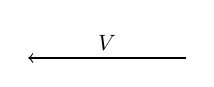
\begin{tikzpicture}
\draw[->] (2,0)-- (0,0) node[pos=0.5,above,scale=0.8] {$V$};
\end{tikzpicture}
$$
%%%%%%%%%%%%%%%%%%%%%%%%%%
\caption{Local relations for colored graphs.
%%   Here $\ph\cc{X}\psi$ denotes the morphism
%% $1 \xrightarrow{\ph \otimes \psi} 
%% V_1 \otimes \cdots \otimes V_n \otimes X \otimes X^* \otimes W_1 \otimes \cdots \otimes W_m  \xrightarrow{ev_{X^*}} 
%% V_1 \otimes \cdots \otimes V_n \otimes W_1 \otimes \cdots \otimes W_m $
%% . 
        }\label{f:local_rels1}
\end{figure}

    Local relations should be understood as follows: for any pair 
    $\Ga, \Ga'$ of colored graphs which are identical  outside a subdisk 
	$D'\subset D$, and in this disk are homeomorphic to the graphs
    shown in  \firef{f:local_rels1},  we must have $\<\Ga\>=\<\Ga'\>$. 
   \end{enumerate}

    Moreover, so defined $\<\Ga\>$ satisfies the following properties:
    \begin{enumerate} 
    \item $\<\Ga\>$ is linear in color of each vertex $v$ \textup{(}for 
         fixed colors of edges and other vertices\textup{)}.
    \item $\<\Ga\>$ is additive in colors of edges as shown in 
          \firef{f:linearity}.

\begin{figure}[ht]
$$
%%%%%%%%%%%%
\begin{tikzpicture}
\node[morphism] (ph) at (0,0) {$\ph$};
\node[morphism] (psi) at (1.5,0) {$\psi$};
\node at (-0.7,0.1) {$\vdots$};
\node at (2.2,0.1) {$\vdots$};
\draw[->] (ph)-- +(220:1cm) node[pos=1.0,below,scale=0.8] {$V_n$};
\draw[->] (ph)-- +(140:1cm) node[pos=1.0,above,scale=0.8] {$V_1$};
\draw[->] (psi)-- +(40:1cm) node[pos=1.0,above,scale=0.8] {$W_m$};
\draw[->] (psi)-- +(-40:1cm) node[pos=1.0,below,scale=0.8] {$W_1$};
\draw[->] (ph) -- (psi) node[pos=0.5,above,scale=0.8] {$X_1\oplus X_2$};
\end{tikzpicture}
%%%%%%%%%%%%
=
%%%%%%%%%%%%
\begin{tikzpicture}
\node[morphism] (ph) at (0,0) {$\ph_1$};
\node[morphism] (psi) at (1.5,0) {$\psi_1$};
\node at (-0.7,0.1) {$\vdots$};
\node at (2.2,0.1) {$\vdots$};
\draw[->] (ph)-- +(220:1cm) node[pos=1.0,below,scale=0.8]{$V_n$};
\draw[->] (ph)-- +(140:1cm) node[pos=1.0,above,scale=0.8]{$V_1$};
\draw[->] (psi)-- +(40:1cm) node[pos=1.0,above,scale=0.8]{$W_m$};
\draw[->] (psi)-- +(-40:1cm) node[pos=1.0,below,scale=0.8]{$W_1$};
\draw[->] (ph) -- (psi) node[pos=0.5,above,scale=0.8] {$X_1$};
\end{tikzpicture}
%%%%%%%%%%%%
+
%%%%%%%%%%%%
\begin{tikzpicture}
\node[morphism] (ph) at (0,0) {$\ph_2$};
\node[morphism] (psi) at (1.5,0) {$\psi_2$};
\node at (-0.7,0.1) {$\vdots$};
\node at (2.2,0.1) {$\vdots$};
\draw[->] (ph)-- +(220:1cm) node[pos=1.0,below,scale=0.8]{$V_n$};
\draw[->] (ph)-- +(140:1cm) node[pos=1.0,above,scale=0.8]{$V_1$};
\draw[->] (psi)-- +(40:1cm) node[pos=1.0,above,scale=0.8]{$W_m$};
\draw[->] (psi)-- +(-40:1cm) node[pos=1.0,below,scale=0.8]{$W_1$};
\draw[->] (ph) -- (psi) node[pos=0.5,above,scale=0.8] {$X_2$};
\end{tikzpicture}
%%%%%%%%%%%%
$$
\caption{Linearity of $\<\Ga\>$. Here $\ph_1,\ph_2$ are compositions
of $\ph$ with projector $X_1\oplus X_2\to X_1$ (respectively, 
$X_1\oplus X_2\to X_2$), and similarly for $\psi_1,\psi_2$.
}\label{f:linearity}
\end{figure}
    \item If $\Ga,\Ga'$ are two isomorphic colorings of the same graph,
      then $\<\Ga\>=\<\Ga'\>$. 
    
    \item Composition property: if $D'\subset D$ is a subdisk such
      that $\del D'$ does not contain vertices of $\Ga$ and meets edges of
      $\Ga$ transversally, then   $\<\Ga\>_D$ will not change if we replace
      subgraph $\Ga\cap D'$ by a single vertex colored by
      $\<\Ga\cap D'\>_{D'}$.

  \end{enumerate}
The vector $\<\Ga\>$ is called the {\em evaluation} of $\Ga$.
\end{thrm}

To define local relations between embedded graphs, Kirillov defines the space of null graphs as follows. Let
$\Ga=c_1\Ga_1+\dots+c_n\Ga_n$ be a formal linear
combination of colored graphs in $\Si$.  If there exists an embedded disk $D \subset M$ such that
\begin{enumerate}
  \item $\Ga$ is transversal to $\del D$ (i.e., no vertices of $\Ga_i$ 
      are on the boundary of $D$ and edges of each $\Ga_i$ meet 
      $\del D$ transversally),
  \item all $\Ga_i$ coincide outside of $D$,
  \item and $\<\Ga\>_D=\sum c_i\<\Ga_i\cap D\>_D=0$;
\end{enumerate}
then $\Ga$ is called a null graph. 




\begin{defn}
The vector space $H := \Hs(\Si, \VV)$ associated to a oriented surface $\Si$ with boundary condition $\VV$ by the spherical fusion category $\mathcal A$ is the quotient space
 $$
   \Hs(\Si, \VV)=\VGr(\Si, \VV)/N(\Si, \VV)
  $$
  where $N(\Si, \VV)$ is  the subspace spanned by null graphs 
  (for all possible embedded disks  $D \subset \Si$). 
\end{defn}
%% The action of the mapping class group on H


%% TODO: \subsection{Birman's mapping class group generators}




\subsection{Strictification}
The colored graph construction takes a strict pivotal category as input, so we must strictify $\Vect_G^\omega$ to get an equivalent strict pivotal monoidal $\widehat \vgo$. Every pivotal category is equivalent to a strict pivotal monoidal category by first strictifying with respect to the monoidal structure, and then strictifying with respect to the pivotal structure as follows \cite{ns}.

Given a monoidal category $\mC$, there exists a monoidally equivalent strict monoidal category $\mC'$ with objects consisting of all finite lists of objects of $\mC$ and morphisms defined by $$\Hom_{\mC'}([A_1, \ldots, A_n], [B_1, \ldots, B_m]) = \Hom_\mC(((\cdots((A_1 \otimes A_2) \otimes A_3) \otimes \cdots \otimes A_n, ((\cdots((B_1 \otimes B_2) \otimes B_3) \otimes \cdots \otimes B_m)$$.  The tensor product in $\mC'$ is concatenation of lists. The strictification functor applies the obvious unique composition of associators to both objects and morphisms of $\mC$, and the coherence map does the same. If $\mC$ is pivotal, this monoidal equivalence extends to an equivalence of pivotal monoidal categories (where the pivotal structure on $\mC'$ is given by applying the strictification functor to the pivotal structure of $\mC$).

Given a pivotal strict monoidal category $\mC'$, there is a strict pivotal monoidal category $\widehat \mC$ equivalent, as a pivotal monoidal category, to $\mC'$.  The objects of $\widehat \mC$ are pairs $(X, \epsilon)$ for which there exists $r \in \NN_0$ such that $X \in \mC^r$ and $\epsilon \in \ZZ_2^r$. The morphisms are
$$\Hom_{\widehat \mC}((X, \epsilon), (Y, \epsilon)) = \Hom_{\mC'}(X_1^{\epsilon_1} \otimes \cdots \otimes X_r^{\epsilon_r}, Y_1^{\epsilon_1} \otimes \cdots \otimes Y_s^{\epsilon_s}),$$
where $X^\epsilon$ is defined by $X^0 = X$ and $X^1 = X^*$. The tensor product is given by concatenation. The duality functor on $\widehat \mC$ is given by
$$(X, \epsilon)^* = ((X_r, \ldots, X_1), (\epsilon_r + 1, \ldots, \epsilon_1 + 1)).$$
The evaluation function $\ev_{(X, \epsilon)}$ on $\widehat \mC$ is inductively defined using tensor products of identities, $j_{X_i}$'s, and evaluation maps $\ev_{X_i}$ in $\mC'$, and similarly for coevaluation.  This strictification functor maps $X \in \mC'$ to $(X, 0)$ and acts on morphisms as the identity.  The coherence maps are also identity maps.

Slightly abusing notation, we will sometimes use the same symbol for both $X \in \mC$ and its images in $\mC'$ and $\widehat \mC$ under the strictification functors.

